%============================================================
\section{Nombre de la habilidad: Luvia de rocas.} \label{hab.LLuviaRocas}
\subsection{Descripción}
Con un poderoso rugido se provoca una lluvia de rocas. Las rocas se destruyen al colisionar con el suelo, con una plataforma o con el jugador. Cuando las rocas colisionan con el jugador disminuyen la cantidad de la barra de vida del jugador. Las rocas no pueden destruir las plataformas o el suelo al colisionar contra estas.
\subsection{Portador}
Tepeyóllotl (ver apartado \ref{per:tepeyollotl}), Mictlantecutli (ver apartado \ref{per:mictlantecutli})..
\subsection{Esquema}
			Ver figura \ref{fig:lluviaR}.
			\begin{figure}
				\centering
				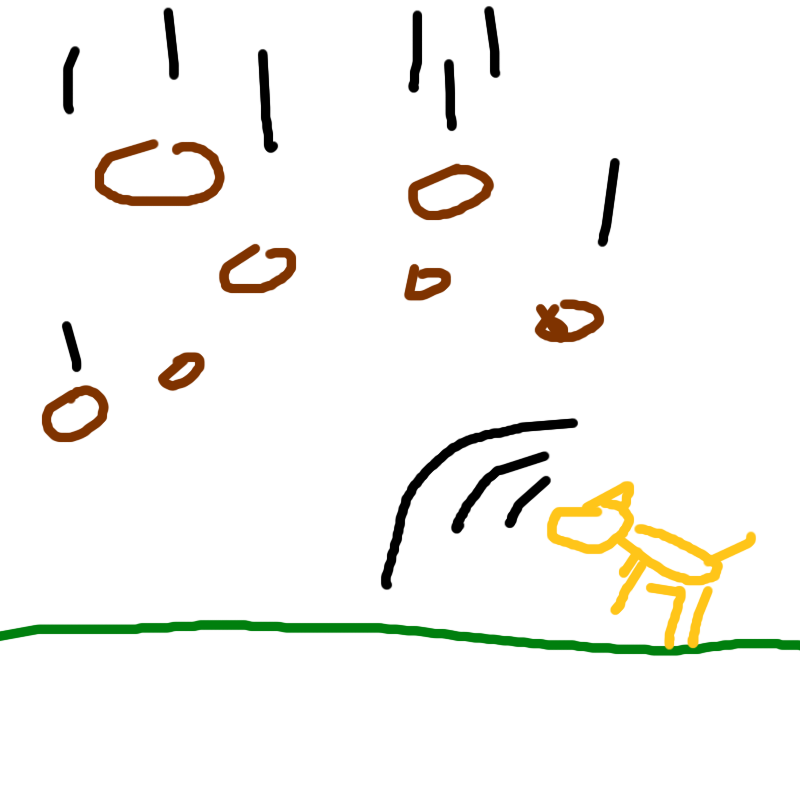
\includegraphics[height=0.2 \textheight]{Imagenes/lluviaR}
				\caption{Lluvia de rocas.}
				\label{fig:lluviaR}
			\end{figure}